%%%%%%%%%%%%%%%%%%%%%%%%%%%%%%%%%%%%%%%%%%%%%%%%%%%%%%%%%%%%%%%%%%%%%%%%%%%%%%%%%%%%%%%%%%%%%%%%%%%%%%
%
%   Filename    : appendix_publications.tex
%
%   Description : The proponent's three papers, reproduced in full at the adviser's request (15 Nov 2026).
%                 Placed between the ethics documents and the resource persons, so it is Appendix B.
%                 Section 5.1 summarizes the papers in the same order. Statuses are the proponent's
%                 (15 Nov 2026): PERSUASIVE published (LNCS, DOI checked on Crossref); TENCON presented
%                 but not yet published, marked "Accepted for publication" at the proponent's request;
%                 ICCE accepted for presentation. Before the final thesis is deposited online, check the publishers'
%                 rules for reusing the papers (IEEE asks for a credit line and the accepted version).
%
%%%%%%%%%%%%%%%%%%%%%%%%%%%%%%%%%%%%%%%%%%%%%%%%%%%%%%%%%%%%%%%%%%%%%%%%%%%%%%%%%%%%%%%%%%%%%%%%%%%%%%

\chapter{Publications}
\label{sec:publications}

This appendix reproduces the three papers summarized in Section~\ref{sec:prelimwork}, in the order in which they are summarized there. Table~\ref{tab:publications} lists them.

\begin{table}[h]
   \centering
   \caption{Papers reproduced in this appendix}
   \label{tab:publications}
   \small
   \begin{tabular}{llL{2.6cm}c}
      \toprule
      Paper & Venue & Status & Section \\
      \midrule
      \citeA{sityar2026persuasive} & PERSUASIVE 2026 & Published & \ref{sec:daisee} \\
      \citeA{carandang2026tencon} & TENCON 2026 & Accepted for publication & \ref{sec:daisee} \\
      \citeA{sityar2026icce} & ICCE 2026 & Accepted for presentation & \ref{sec:prelim} \\
      \bottomrule
   \end{tabular}
\end{table}

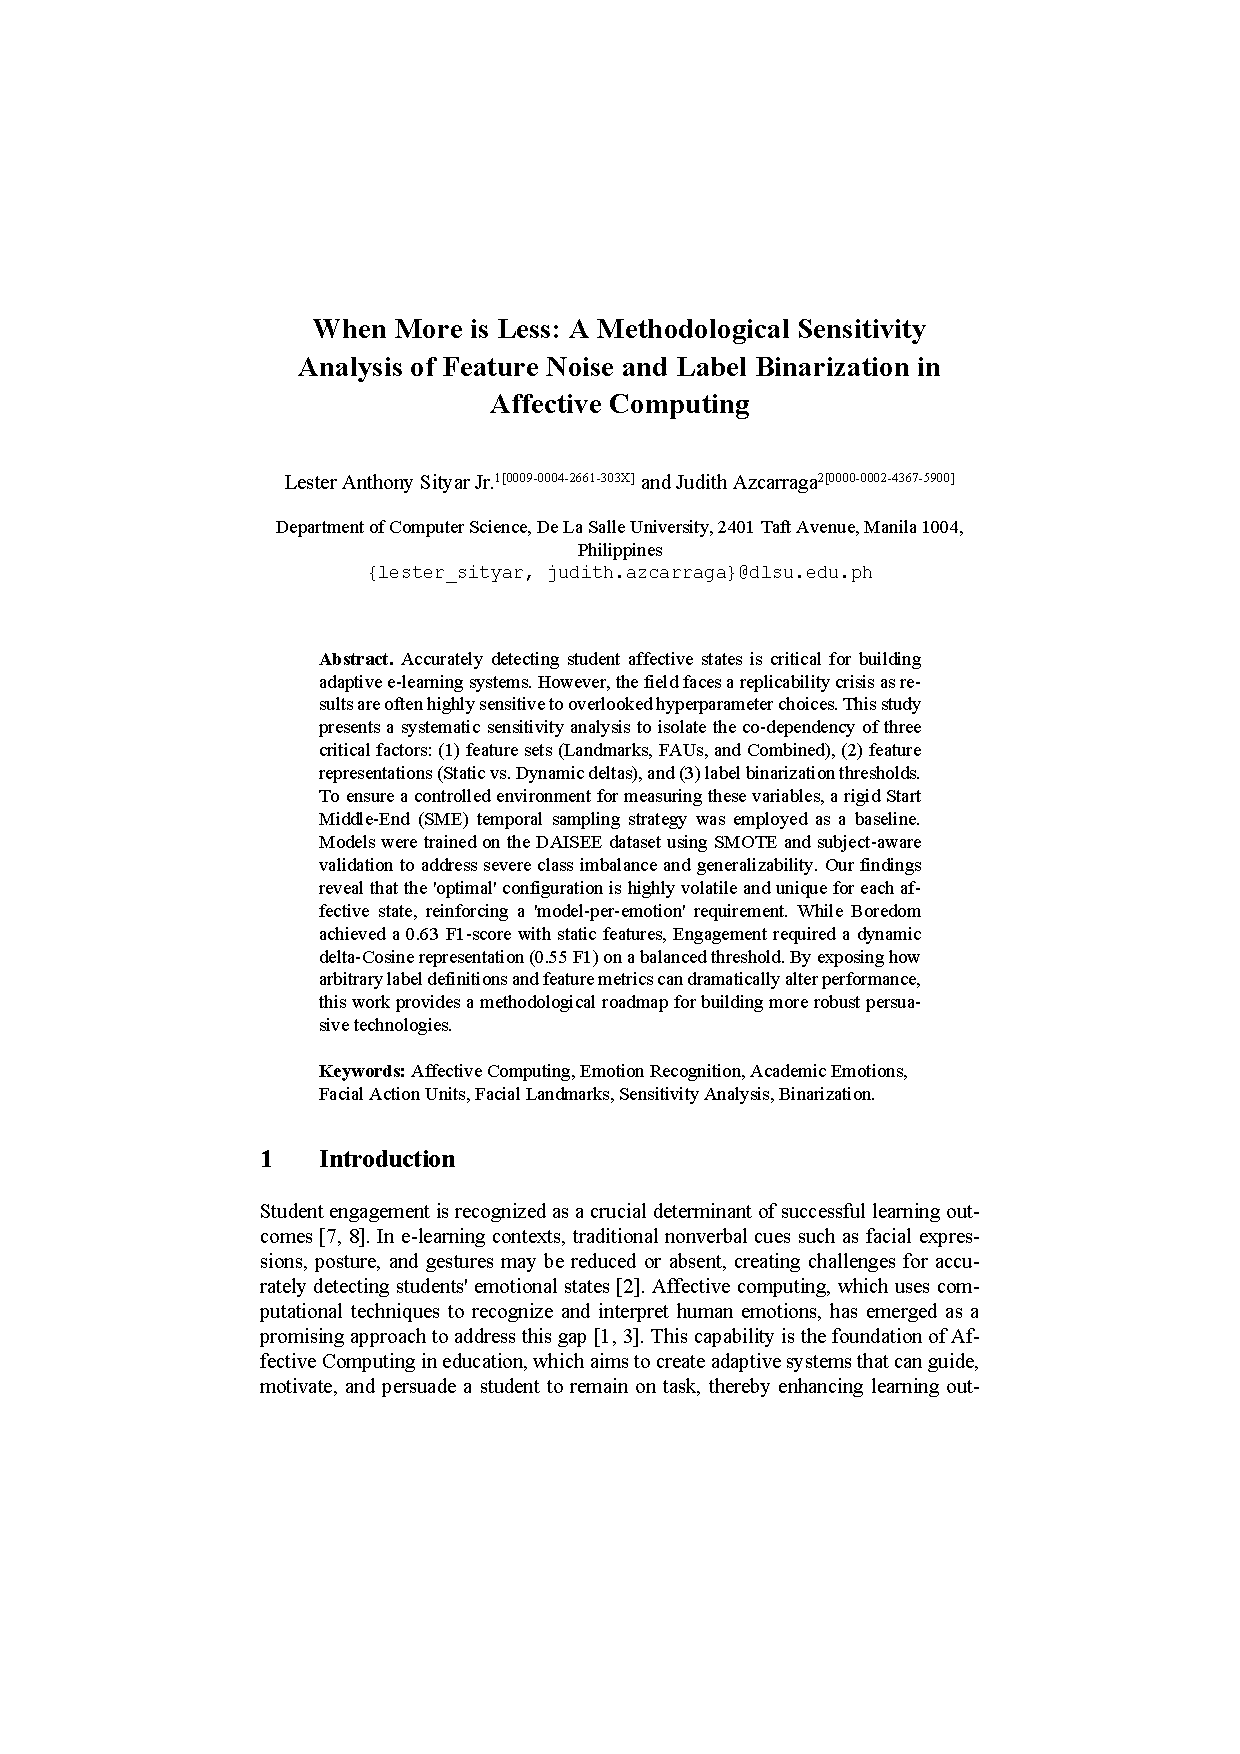
\includepdf[pages=-, scale=0.9, pagecommand={}, offset=-30 0,
   addtotoc={1, section, 1, {When More is Less (PERSUASIVE 2026)}, sec:pub-persuasive}]
   {past-papers/SITYAR-PERSUASIVE2026-Paper.pdf}

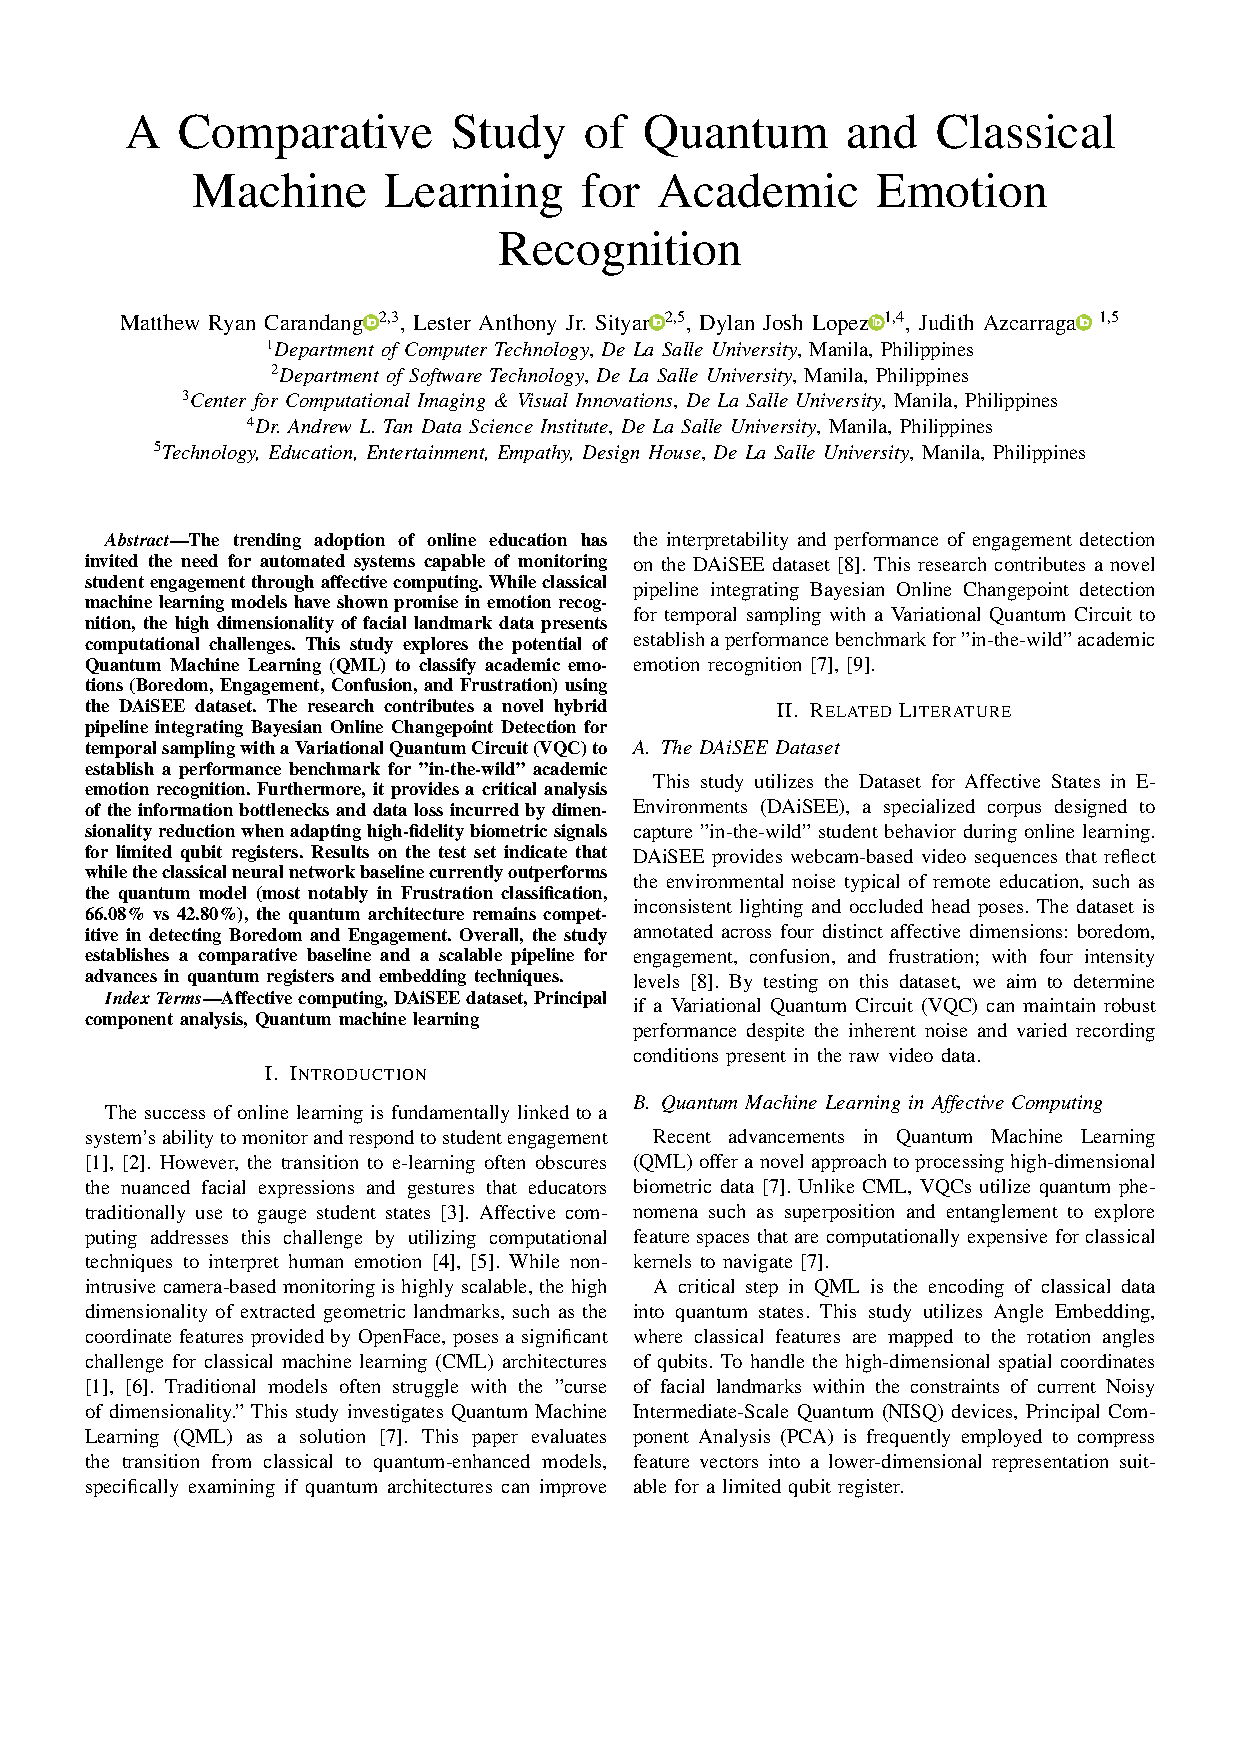
\includepdf[pages=-, scale=0.9, pagecommand={}, offset=-30 0,
   addtotoc={1, section, 1, {A Comparative Study of Quantum and Classical Machine Learning (TENCON 2026)}, sec:pub-tencon}]
   {past-papers/SITYAR-TENCON2026-Paper.pdf}

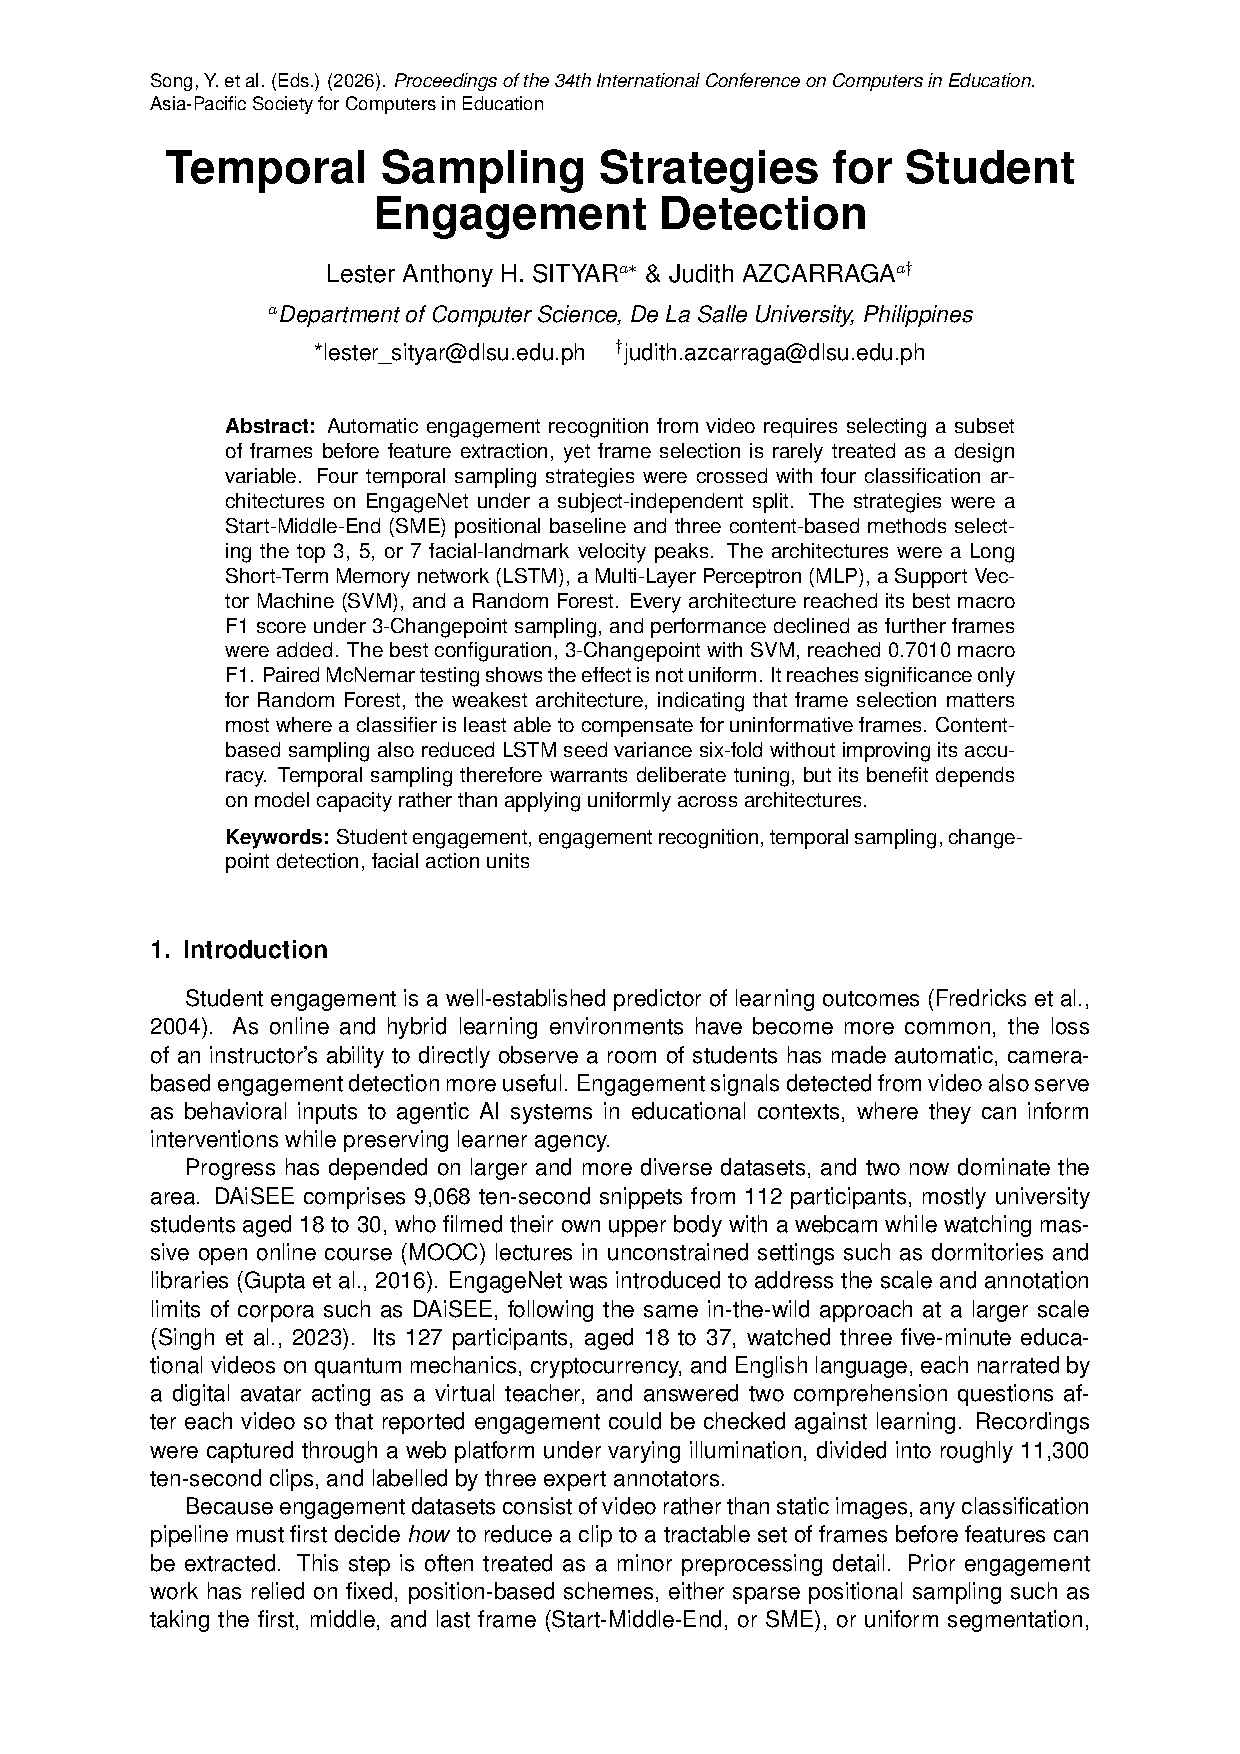
\includepdf[pages=-, scale=0.9, pagecommand={}, offset=-30 0,
   addtotoc={1, section, 1, {Temporal Sampling Strategies for Student Engagement Detection (ICCE 2026)}, sec:pub-icce}]
   {past-papers/SITYAR-ICCE2026-Paper.pdf}
